\documentclass[12pt]{article}
%NOTE: This report format is 

\newcommand{\reporttitle}{Rapport de Projet : Régulation d’un bâtiment thermiquement actif}
\newcommand{\reportauthorOne}{Benjamin BOCK}
\newcommand{\cidOne}{S2304467}
\newcommand{\reportauthorTwo}{Odayfa DAKIR}
\newcommand{\cidTwo}{S23XXXXX}
\newcommand{\reportauthorThree}{Yazan SALOUM}
\newcommand{\cidThree}{S23XXXXX}
\newcommand{\reporttype}{Coursework}
\bibliographystyle{plain}

% include files that load packages and define macros
\usepackage{fontspec}
\usepackage{newtxtext,newtxmath} % Times New Roman pour texte et maths



% Packages utiles (ajoutez ceux dont vous avez besoin)
\usepackage[letterpaper,hmargin=2.8cm,vmargin=2.0cm,includeheadfoot]{geometry}
\usepackage{textpos}
\usepackage{natbib}
\usepackage{stackengine}
\usepackage{tabularx,longtable,multirow,subfigure,caption}%hangcaption
\usepackage{fncylab} %formatting of labels
\usepackage{fancyhdr}
\usepackage{color}
\usepackage[tight,ugly]{units}
\usepackage{url}
\usepackage{float}
\usepackage[english]{babel}
\usepackage{amsmath}
\usepackage{graphicx}
\usepackage[colorinlistoftodos]{todonotes}
\usepackage{dsfont}
\usepackage{epstopdf} % automatically replace .eps with .pdf in graphics
\usepackage{backref}
\usepackage{array}
\usepackage{etoolbox}
\usepackage{enumerate} % for numbering with [a)] format 
\usepackage{tcolorbox}
\usepackage{graphicx} % Pour insérer des images
\usepackage{tocloft}  % Pour personnaliser la liste des figures


% table of content
\renewcommand{\tableofcontentsname}{Table of Contents}

% table of figures
\renewcommand{\listfigurename}{Table of Figures}

% various theorems
\usepackage{ntheorem}
\theoremstyle{break}
\newtheorem{lemma}{Lemma}
\newtheorem{theorem}{Theorem}
\newtheorem{remark}{Remark}
\newtheorem{definition}{Definition}
\newtheorem{proof}{Proof}

% example-environment
\newenvironment{example}[1][]
{ 
\vspace{4mm}
\noindent\makebox[\linewidth]{\rule{\hsize}{1.5pt}}
\textbf{Example #1}\\
}
{ 
\noindent\newline\makebox[\linewidth]{\rule{\hsize}{1.0pt}}
}

\setlength{\parindent}{0em}  % indentation of paragraph

\setlength{\headheight}{14.5pt}
\pagestyle{fancy}
\fancyfoot[ER,OR]{\thepage}%Page no. in the left on
                                %odd pages and on right on even pages
\fancyfoot[OC,EC]{\sffamily }
\renewcommand{\headrulewidth}{0.1pt}
\renewcommand{\footrulewidth}{0.1pt}
\captionsetup{margin=10pt,font=small,labelfont=bf}

%--- chapter heading
\def\@makechapterhead#1{%
  \vspace*{10\p@}%
  {\parindent \z@ \raggedright
    \interlinepenalty\@M
    \Huge \bfseries 
    \thechapter \space\space #1\par\nobreak
    \vskip 30\p@
  }}

%---chapter heading for \chapter*  
\def\@makeschapterhead#1{%
  \vspace*{10\p@}%
  {\parindent \z@ \raggedright
    \interlinepenalty\@M
    \Huge \bfseries  
    #1\par\nobreak
    \vskip 30\p@
  }}

% %%%%%%%%%%%%% boxit
\def\Beginboxit
   {\par
    \vbox\bgroup
	   \hrule
	   \hbox\bgroup
		  \vrule \kern1.2pt %
		  \vbox\bgroup\kern1.2pt
   }

\def\Endboxit{%
			      \kern1.2pt
		       \egroup
		  \kern1.2pt\vrule
		\egroup
	   \hrule
	 \egroup
   }	

\newenvironment{boxit}{\Beginboxit}{\Endboxit}
\newenvironment{boxit*}{\Beginboxit\hbox to\hsize{}}{\Endboxit}

\allowdisplaybreaks

\makeatletter
\newcounter{elimination@steps}
\newcolumntype{R}[1]{>{\raggedleft\arraybackslash$}p{#1}<{$}}
\def\elimination@num@rights{}
\def\elimination@num@variables{}
\def\elimination@col@width{}
\newenvironment{elimination}[4][0]
{
    \setcounter{elimination@steps}{0}
    \def\elimination@num@rights{#1}
    \def\elimination@num@variables{#2}
    \def\elimination@col@width{#3}
    \renewcommand{\arraystretch}{#4}
    \start@align\@ne\st@rredtrue\m@ne
}
{
    \endalign
    \ignorespacesafterend
}
\newcommand{\eliminationstep}[2]
{
    \ifnum\value{elimination@steps}>0\leadsto\quad\fi
    \left[
        \ifnum\elimination@num@rights>0
            \begin{array}
            {@{}*{\elimination@num@variables}{R{\elimination@col@width}}
            |@{}*{\elimination@num@rights}{R{\elimination@col@width}}}
        \else
            \begin{array}
            {@{}*{\elimination@num@variables}{R{\elimination@col@width}}}
        \fi
            #1
        \end{array}
    \right]
    & 
    \begin{array}{l}
        #2
    \end{array}
    &%                                    moved second & here
    \addtocounter{elimination@steps}{1}
}
\makeatother

%% Fast macro for column vectors
\makeatletter  
\def\colvec#1{\expandafter\colvec@i#1,,,,,,,,,\@nil}
\def\colvec@i#1,#2,#3,#4,#5,#6,#7,#8,#9\@nil{% 
  \ifx$#2$ \begin{bmatrix}#1\end{bmatrix} \else
    \ifx$#3$ \begin{bmatrix}#1\\#2\end{bmatrix} \else
      \ifx$#4$ \begin{bmatrix}#1\\#2\\#3\end{bmatrix}\else
        \ifx$#5$ \begin{bmatrix}#1\\#2\\#3\\#4\end{bmatrix}\else
          \ifx$#6$ \begin{bmatrix}#1\\#2\\#3\\#4\\#5\end{bmatrix}\else
            \ifx$#7$ \begin{bmatrix}#1\\#2\\#3\\#4\\#5\\#6\end{bmatrix}\else
              \ifx$#8$ \begin{bmatrix}#1\\#2\\#3\\#4\\#5\\#6\\#7\end{bmatrix}\else
                 \PackageError{Column Vector}{The vector you tried to write is too big, use bmatrix instead}{Try using the bmatrix environment}
              \fi
            \fi
          \fi
        \fi
      \fi
    \fi
  \fi 
}  
\makeatother

\robustify{\colvec} % various packages needed for maths etc.
% quick way of adding a figure
\newcommand{\fig}[3]{
 \begin{center}
 \scalebox{#3}{\includegraphics[#2]{#1}}
 \end{center}
}

%\newcommand*{\point}[1]{\vec{\mkern0mu#1}}
\newcommand{\ci}[0]{\perp\!\!\!\!\!\perp} % conditional independence
\newcommand{\point}[1]{{#1}} % points 
\renewcommand{\vec}[1]{{\boldsymbol{{#1}}}} % vector
\newcommand{\mat}[1]{{\boldsymbol{{#1}}}} % matrix
\newcommand{\R}[0]{\mathds{R}} % real numbers
\newcommand{\Z}[0]{\mathds{Z}} % integers
\newcommand{\N}[0]{\mathds{N}} % natural numbers
\newcommand{\nat}[0]{\mathds{N}} % natural numbers
\newcommand{\Q}[0]{\mathds{Q}} % rational numbers
\ifxetex
\newcommand{\C}[0]{\mathds{C}} % complex numbers
\else
\newcommand{\C}[0]{\mathds{C}} % complex numbers
\fi
\newcommand{\tr}[0]{\text{tr}} % trace
\renewcommand{\d}[0]{\mathrm{d}} % total derivative
\newcommand{\inv}{^{-1}} % inverse
\newcommand{\id}{\mathrm{id}} % identity mapping
\renewcommand{\dim}{\mathrm{dim}} % dimension
\newcommand{\rank}[0]{\mathrm{rk}} % rank
\newcommand{\determ}[1]{\mathrm{det}(#1)} % determinant
\newcommand{\scp}[2]{\langle #1 , #2 \rangle}
\newcommand{\kernel}[0]{\mathrm{ker}} % kernel/nullspace
\newcommand{\img}[0]{\mathrm{Im}} % image
\newcommand{\idx}[1]{{(#1)}}
\DeclareMathOperator*{\diag}{diag}
\newcommand{\E}{\mathds{E}} % expectation
\newcommand{\var}{\mathds{V}} % variance
\newcommand{\gauss}[2]{\mathcal{N}\big(#1,\,#2\big)} % gaussian distribution N(.,.)
\newcommand{\gaussx}[3]{\mathcal{N}\big(#1\,|\,#2,\,#3\big)} % gaussian distribution N(.|.,.)
\newcommand{\gaussBig}[2]{\mathcal{N}\left(#1,\,#2\right)} % see above, but with brackets that adjust to the height of the arguments
\newcommand{\gaussxBig}[3]{\mathcal{N}\left(#1\,|\,#2,\,#3\right)} % see above, but with brackets that adjust to the height of the arguments
\DeclareMathOperator{\cov}{Cov} % covariance (matrix) 
\ifxetex
\renewcommand{\T}[0]{^\top} % transpose
\else
\newcommand{\T}[0]{^\top}
\fi
% matrix determinant
\newcommand{\matdet}[1]{
\left|
\begin{matrix}
#1
\end{matrix}
\right|
}



%%% various color definitions
\definecolor{darkgreen}{rgb}{0,0.6,0}

\newcommand{\blue}[1]{{\color{blue}#1}}
\newcommand{\red}[1]{{\color{red}#1}}
\newcommand{\green}[1]{{\color{darkgreen}#1}}
\newcommand{\orange}[1]{{\color{orange}#1}}
\newcommand{\magenta}[1]{{\color{magenta}#1}}
\newcommand{\cyan}[1]{{\color{cyan}#1}}


% redefine emph
\renewcommand{\emph}[1]{\blue{\bf{#1}}}

% place a colored box around a character
\gdef\colchar#1#2{%
  \tikz[baseline]{%
  \node[anchor=base,inner sep=2pt,outer sep=0pt,fill = #2!20] {#1};
    }%
}%
 % short-hand notation and macros


%%%%%%%%%%%%%%%%%%%%%%%%%%%%

\begin{document}
% front page
% Last modification: 2016-09-29 (Marc Deisenroth)
% Modification for UW: 2017-05-22 (jphickey)
\begin{titlepage}

\newcommand{\HRule}{\rule{\linewidth}{0.5mm}} % Defines a new command for the horizontal lines, change thickness here


%----------------------------------------------------------------------------------------
%	LOGO SECTION
%----------------------------------------------------------------------------------------



\begin{center} % Center remainder of the page

%----------------------------------------------------------------------------------------
%	HEADING SECTIONS
%----------------------------------------------------------------------------------------


\includegraphics[width = 15cm]{./figures/uliege_faculte_sciencesappliquees_logo_rvb}\\[1.5cm] 
\textbf{\textsc{\Large PROJ0001-1 Introduction \\
aux méthodes numériques et projet}}\\[1.0cm] 
\textsc{\Large Université de Liège}\\[0.5cm] 
\textsc{\large Faculté des Sciences Appliquées}\\[0.45cm] 
\textsc{\large Année académique 2024-2025}\\[0.45cm] 


%----------------------------------------------------------------------------------------
%	TITLE SECTION
%----------------------------------------------------------------------------------------

\HRule \\[0.4cm]
{ \huge \bfseries \reporttitle}\\ % Title of your document
\HRule \\[1.5cm]
\end{center}
%----------------------------------------------------------------------------------------
%	AUTHOR SECTION
%----------------------------------------------------------------------------------------

%\begin{minipage}{0.4\hsize}

\begin{center}
    \begin{minipage}{0.45\linewidth} % Bloc à gauche
        \raggedright % Aligné à gauche
        \normalsize \textit{Professeurs:} \\
            \small  Olivier BRULS \\
                    Quentin LOUVEAUX \\
                    Frédéric NGUYEN 
    \end{minipage}
    \begin{minipage}{0.45\linewidth} % Bloc à droite
        \raggedleft % Aligné à droite
        \normalsize \textit{Auteurs:} \\
        \begin{small}
            \reportauthorOne~(\cidOne)\\
            \reportauthorTwo~(\cidTwo)\\
            \reportauthorThree~(\cidThree)\\
        \end{small}
    \end{minipage}
\end{center}


\vspace{4cm}
\makeatletter
Liège, le \today

\vfill % Fill the rest of the page with whitespace



\makeatother

\end{titlepage}




%%%%%%%%%%%%%%%%%%%%%%%%%%% table of content
%If a table of content is needed, simply uncomment the following lines
\renewcommand{\contentsname}{Table des matières}
\renewcommand{\listfigurename}{Table des figures}
\tableofcontents
\newpage
\listoffigures
\newpage


%%%%%%%%%%%%%%%%%%%%%%%%%%%% Main document
\section{Introduction}
cc
\section{Summary of the problem}


To tie-in the concepts seen in ME303, we will turn our attention to the fascinating physical phenomenon of sonoluminescence. This occurs when a single bubble, usually of micrometer in size, within a liquid emits a short burst of light when imploding under an externally excited acoustic source. As the energy is concentrated into a point source, local temperatures in the collapsing bubble can reach up to 10,000 K for up to 50 pico seconds and visible light is emitted.

The origin of the light emission is an unsolved physical problem and obviously outside the scope of ME303. For project 1, we will be studying the governing equations behind the bubble oscillation leading up to a the light burst.
\begin{figure}[h!]
\centering
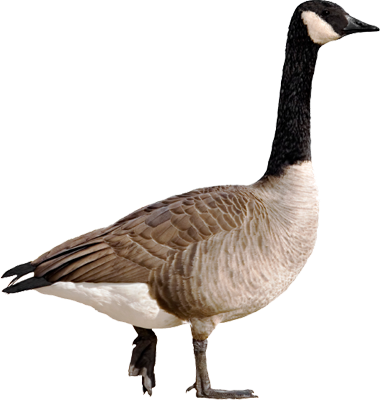
\includegraphics[width=0.45\textwidth]{figures/goose.png} 
\caption{A goose.}
\label{goose}
\end{figure}


The radius of a bubble under a varying pressure field is defined by the Rayleigh-Plesset equation. This equation is derived using standard conservation law under a number of simplifying assumptions:
\begin{equation}
\rho_l \left(R\ddot{R} + \frac{3}{2}\dot{R}^2\right) = p_{gas} -P(t) -P_0 +\frac{R}{c}\frac{d p_{gas}}{dt} - 4\mu \frac{\dot{R}}{R}-\frac{2\sigma}{R}
\label{RP}
\end{equation}
In the above equation $R(t)$ [m] represents the bubble radius. The other terms are: $\rho_l$ [$kg\cdot m^3$]  the density of the liquid, $p_{gas}$ [Pa] the pressure of the gas inside the bubble, $P(t)$ [Pa] the imposed oscillatory pressure field, $P_0$ [Pa] the baseline pressure, $c$ [$m/s$] speed of sound in the liquid, $\mu$ [$Pa\cdot s$] molecular viscosity of the liquid and $\sigma$ [$kg\cdot s^{-2}$] the surface tension at the bubble-water interface.

For more contextual information on the bubble dynamic phenomena, please see the following sources: \cite{Hilgenfeldt1998}, \cite{Kreider2011}, and \cite{Lohse2003}.



\section{Questions}
\emph{This section answers the individual questions of the project description.  For each question, provide an answer and short analysis.}
\subsection*{Question 1: Forced bubble oscillation}
\subsubsection*{(a)} \emph{References to equations can be written out in latex \eqref{RP}. Similarly, figures  \ref{goose} and sections \ref{Q2} may also be referenced.}
\subsubsection*{(b)} \emph{Citations require the mybib.tex file to be extended with the desired references. Students can use JabRef (\url{http://www.jabref.org}) to construct the mybib.bib file. Students are invited to link their Mendelay, CiteULike and Zotero account directly to Overleaf. }

\subsection{Question 2: Bubble evolution \label{Q2}}


\vfill

\section*{Students' contributions}
Mr. Goose and Mrs. Goose worked together to understand the problem and write the numerical codes. The summary of the problem and Q2 were written up by Mr. Goose, Q1 and Q3 were completed by Mrs. Goose. Both students corrected the final report.

\newpage
\bibliography{mybib}


\end{document}
%%% Local Variables: 
%%% mode: latex
%%% TeX-master: t
%%% End: 
